\documentclass[11pt]{article}

% Margins ----------------------------------------------------------------------
\usepackage[margin=1.25in]{geometry}

% Line Spacing -----------------------------------------------------------------
\renewcommand{\baselinestretch}{1.5}

% Font -------------------------------------------------------------------------
\usepackage{utopia}
\usepackage[utopia, smallerops, varg]{newtxmath}
% \usepackage{cabin}
% \usepackage[libertine]{newtxmath}
% \usepackage{Baskervaldx}

% Small adjustments to text kerning
\usepackage{microtype}

% Remove annoying over-full box warnings ---------------------------------------
\vfuzz2pt 
\hfuzz2pt

% Tikz support -----------------------------------------------------------------
\usepackage{tikz}


% Color Palette ----------------------------------------------------------------
\usepackage{xcolor}

% https://www.materialpalette.com/colors
\definecolor{red}{HTML}{c62828}
\definecolor{orange}{HTML}{ef6c00}
\definecolor{green}{HTML}{2e7d32}
\definecolor{blue}{HTML}{1565c0}
\definecolor{purple}{HTML}{283593}
\definecolor{maroon}{HTML}{AF3335}
\definecolor{dark-maroon}{HTML}{5D0F0D}
\definecolor{teal}{HTML}{00695c}
\definecolor{bluegrey}{HTML}{455a64}
\definecolor{indigo}{HTML}{1A237E}
\definecolor{navyblue}{HTML}{0A3044}
\definecolor{bluegreen}{HTML}{4A8676}
\definecolor{Black}{HTML}{000000}

% CU Boulder colors
\definecolor{buff-gold}{HTML}{CFB87C}
\definecolor{buff-grey}{HTML}{565A5C}
\definecolor{buff-lightgrey}{HTML}{A2A4A3}
\definecolor{buff-black}{HTML}{000000}


% Hyperlinks -------------------------------------------------------------------
\usepackage{hyperref}
\hypersetup{
    colorlinks= true,
    citecolor= dark-maroon,
    linkcolor= dark-maroon,
    filecolor= dark-maroon,      
    urlcolor= dark-maroon,
}

% Citations --------------------------------------------------------------------
\usepackage[
    style= authoryear, 
    natbib= true, 
    backend= biber
]{biblatex}


% Enumerate/Itemize ------------------------------------------------------------
\usepackage{enumitem}
\setlist[itemize]{label= \textbullet}

% Section and Subsection Styling -----------------------------------------------
\usepackage[explicit]{titlesec}

\titleformat{\section}
  {\large \bf \color{navyblue}}
  {\thesection \,---}
  {0.25em}
  {#1}
  
\titleformat{\subsection}
  {\fontsize{11}{10}\it}
  {\thesubsection.}
  {1em}
  {#1}

% Footnote ---------------------------------------------------------------------
% Spacing between footnotes on same page
\addtolength{\footnotesep}{1mm}

% Space after footnote number
\let\oldfootnote\footnote
\renewcommand\footnote[1]{\oldfootnote{\ #1}}

% Better Abstract --------------------------------------------------------------
\renewenvironment{abstract}
{
  \centerline
  {\large \bfseries \scshape \color{navyblue} Abstract}
  \begin{quote}
}
{
  \end{quote}
}

% AMS --------------------------------------------------------------------------
\usepackage{amsmath}
\usepackage{amsfonts}
\usepackage{graphicx}


% Table and Figure labelling ---------------------------------------------------
\usepackage{caption}

\DeclareCaptionLabelSeparator{threesdash}{\,---\,}
\DeclareCaptionLabelSeparator{period}{\,---\,}
\captionsetup[table]{format=plain,labelsep=threesdash, font=bf}
\captionsetup[figure]{format=plain, labelsep=period, font=bf}
% Left align captions
% \captionsetup[table]{labelfont=it, textfont={bf}, labelsep=newline, justification=raggedright, singlelinecheck=off}
% \captionsetup[figure]{labelfont=it, textfont={bf}, labelsep=newline, justification=raggedright, singlelinecheck=off}


% Tables -----------------------------------------------------------------------

% Tables too big
% \begin{adjustbox}{width = 1.2\textwidth, center}
\usepackage{adjustbox}
\usepackage{array}

% Slighty more spacing between rows
\renewcommand\arraystretch{1.1}

% Tables too narrow
% \begin{tabularx}{\linewidth}{cols}
% col-types: X - center, L - left, R -right
% Relative scale: >{\hsize=.8\hsize}X/L/R
\usepackage{tabularx}
\newcolumntype{L}{>{\raggedright\arraybackslash}X}
\newcolumntype{R}{>{\raggedleft\arraybackslash}X}
\newcolumntype{C}{>{\centering\arraybackslash}X}

% \begin{threeparttable}
%    \begin{tabular} ... \end{tabular}
%    \begin{tablenotes}
%        \item \textit{Notes.}
%    \end{tablenotes}  
% \end{threeparttable}
\usepackage[flushleft]{threeparttable}
\setlength\labelsep{0pt}

% \toprule, \cmidrule, \bottomrule
\usepackage{booktabs}

% Landscape table --------------------------------------------------------------
% \begin{landscape} \pagestyle{lscaped} table... \end{landscsape}
% \usepackage{pdflscape} - rotates page left-side up in pdf
% \usepackage{lscape} - does not rotate page, only figure/table

\usepackage{pdflscape}
% \usepackage{lscape}

\usepackage{fancyhdr}
\fancypagestyle{lscaped}{%
    \fancyhf{}
    \renewcommand{\headrulewidth}{0pt}
    \textnormal
    \fancyfoot{%
        \tikz[remember picture,overlay]
        \node[outer sep=2.5cm,above,rotate=90] at (current page.east) {\thepage};
    }
}


% Define Theorems --------------------------------------------------------------
% note, theorem is the name that goes in \begin{} and Theorem is the name displayed as Theorem 1
\newtheorem{theorem}{Theorem}


% ------------------------------------------------------------------------------

\usepackage{hyperref}
\usepackage{graphicx}

\date{\today}

\begin{document}

\begin{center}
	{\Large \color{navyblue} \bf ECON 3535: Nautural Resource Economics}
	
	MWF 12:40-1:30
\end{center}

\vspace{.2cm}
\noindent \textbf{Instructor:} Kyle Butts

\noindent \textbf{Email:} \href{mailto:kyle.butts@colorado.edu}{kyle.butts@colorado.edu}

\noindent \textbf{Office Hours:} W 10:30-12:30 and by appointment

\vspace{5mm} \noindent \textit{Please allow me 24 hours to respond to all emails. If you need help with course material, please see me during my office hours. If you need more help than can be provided in office hours, consider visiting the department's undergraduate tutor or viewing the department's private tutor list:} \url{http://www.colorado.edu/econ/undergraduate/tutor_list.pdf}

\section*{Course Description}
This course in natural resource economics will introduce students to the relationship between natural resources and the economic system. Classic allocation problems for renewable and nonrenewable resources will be examined. Understanding the incentives faced by users of natural resources will allow us to consider market failures and the important question of whether or not market interventions are justified on economic grounds. Because natural resources play a central role in many current energy and environmental policy debates, this course will also address institutions and policy issues related to climate change, ecosystem services, renewable energy, transportation, and sustainability.


\section*{Textbook}
I will assign readings from this book and from other sources, all posted on Canvas. I will not ask you to
own a physical copy of the textbook. There is a pdf of the book available for free online.

\textit{Environmental and Natural Resource Economics, 9th Edition}
by Tietenberg and Lewis; ISBN-13: 978-0131392571.



\vspace{5mm}\noindent 
\textbf{Grading}
\begin{center}
	\small{
        \begin{tabular}{| l | c |}
            \hline
            \textbf{Assignment} & \textbf{Percentage}\\ 
			\hline
			Midterm & 30\% \\ \hline
			Assignments & 30\%  \\ \hline
			Final & 40\%  \\ \hline
		\end{tabular}}
\end{center}

We will have two midterms, but I will only count the higher grade of the two. The final exam will be cumulative, but more more heavily weighted towards the most recent material.

I will curve each midterm separately. After the final exam I will curve the final grades so that the average grade for the whole class is an 81 (B-). The curve follows a strict formula, and I will not manually adjust grades for any reason. Letter grades are assigned according to the standard numerical formula used at CU:

\begin{center}
	\footnotesize{
		\begin{tabular}{|c|c|c|c|}
			\hline
			\textbf{Grade} & \textbf{Percentage} & \textbf{Grade} & \textbf{Percentage}       \\ \hline
			A  & $93 \leq x$      & C  & $73 \leq x < 77$ \\ \hline
			A- & $90 \leq x < 93$ & C- & $70 \leq x < 73$ \\ \hline
			B+ & $87 \leq x < 90$ & D+ & $67 \leq x < 70$ \\ \hline
			B  & $83 \leq x < 87$ & D  & $63 \leq x < 67$ \\ \hline
			B- & $80 \leq x < 83$ & D- & $60 \leq x < 63$ \\ \hline
			C+ & $77 \leq x < 80$ & F  & x $< 60$         \\ \hline
		\end{tabular}}
\end{center}

If you have university testing accommodations, let me know well ahead of the exam so that I can set things up to suit your needs.


\section*{Assignments}

There will be one math assignment and one literature review assignment. The math assignment will involve using economic models to solve problems related to natural resource allocation. These will be graded for correctness, and you may work alone or in groups of up to four. Each group will turn in a single assignment and receive a shared grade.

The written assignment will be of a “literature review” format, where you will choose a research question and write a paper discussing the academic literature around that question. I will provide detailed guidelines for this assignment. Literature reviews will be graded based on effort and meeting the guidelines.




\section*{Course Policies}
\textit{Attendance} - I will not be taking attendance, so skip class at your own risk. Lecture slides will be posted on Canvas. The slides are a valuable study tool for the exams, but it will be hard to do well without regular attendance.


\vspace{5mm}\noindent
\textit{Makeups} - There will be no makeup tests, even if your reason for missing the test is very good. If a test conflicts with a mandatory CU event, we can arrange to have you take it before the test day, but not after. Similarly, assignments are given well ahead of their due date, so late assignments will not receive credit.


\vspace{5mm}\noindent
\textit{Email} - Feel free to email me with questions about the course. However, if you want to talk about why you got a particular grade, you must come to office hours. Please give me 24 hours to respond before sending another email.


\vspace{5mm}\noindent
\textit{Office Hours} - If you have a schedule conflict during my office hours, you may email me to set up a different time to meet.


\vspace{5mm}\noindent
\textit{Cheating} - Don’t do it, you will automatically get a zero.

\newpage
\section*{Tentative Course Outline}
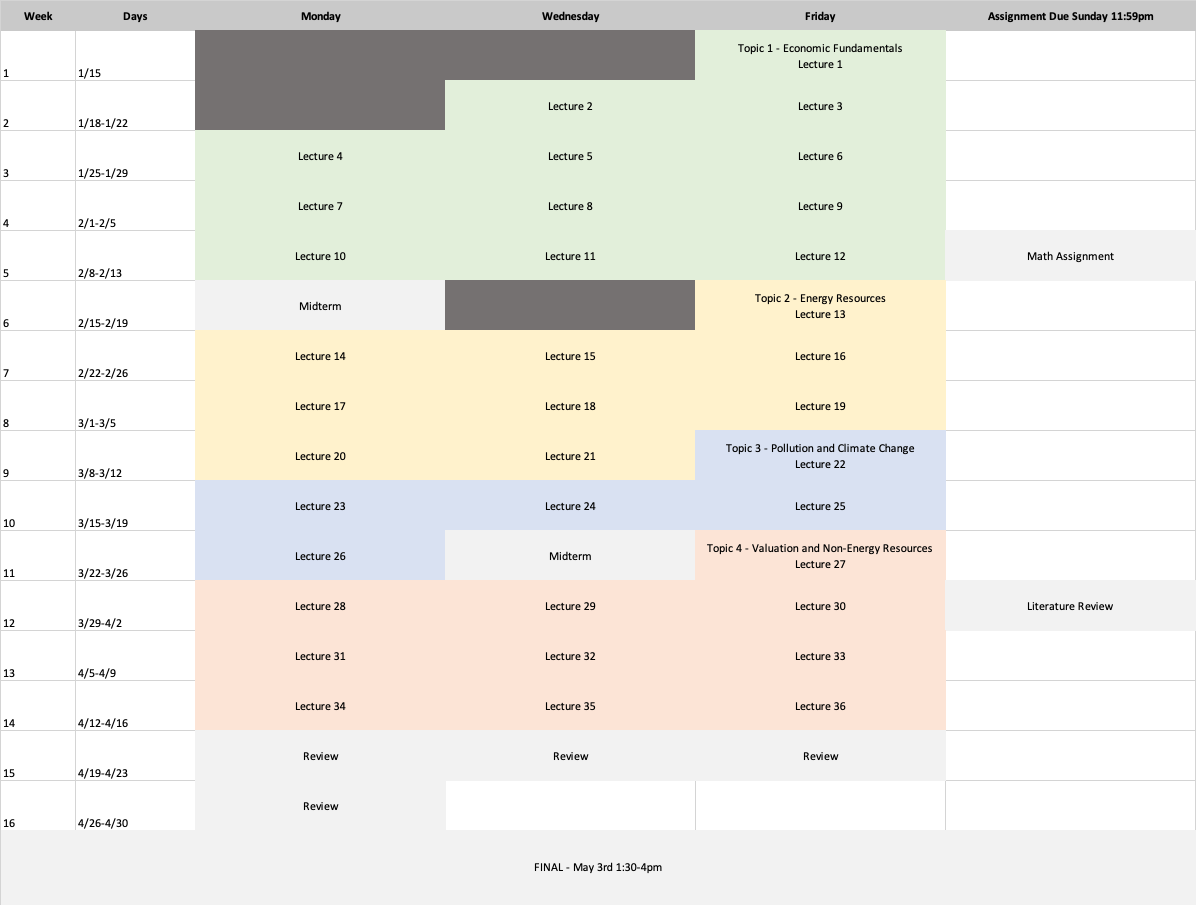
\includegraphics[width=\linewidth]{schedule.png}



\newpage
\section*{University Policies}

\footnotesize{
	\vspace{5mm}\noindent 
	\textbf{Students with Disabilities:} 
	If you qualify for accommodations because of a disability, please submit to me a letter from disability services in a timely manner so that your needs can be addressed. Disability services determine accommodations based on documented disabilities.
	Contact: 303-492-8671, Center for Community N200.
	
	\vspace{5mm}\noindent
	\textbf{Religious Observance Policy:}
	Campus policy regarding religious observances requires that faculty make every effort to reasonably and fairly deal with all students who, because of religious obligations, have conflicts with scheduled exams, assignments, or required attendance. If you have a conflict, please contact me at the beginning of the term so we can make proper arrangements. 
	
	\vspace{5mm}\noindent
	\textbf{Honor Code:}
	All students of the University of Colorado at Boulder are responsible for knowing and adhering to the academic integrity policy of this institution. Violations of this policy may include: cheating, plagiarism, aid of academic dishonesty, fabrication, lying, bribery, and threatening behavior. All incidents of academic misconduct shall be reported to the Honor Code Council (\href{mailto:honor@colorado.edu}{honor@colorado.edu}; 303-725-2273).
	Students who are found to be in violation of the academic integrity policy will be subject to both academic sanctions from the faculty member and non-academic sanctions (including but not limited to university probation, suspension, or expulsion). Other information on the Honor Code can be found at: \url{http://www.colorado.edu/policies/honor.html} and at \url{http://www.colorado.edu/academics/honorcode/}
	
	\vspace{5mm}\noindent
	\textbf{Discrimination \& Harassment Policy:}
	The University of Colorado Policy on Sexual Harassment applies to all students, staff and faculty. Sexual harassment is unwelcome sexual attention. It can involve intimidation, threats, coercion, or promises or create an environment that is hostile or offensive. Harassment may occur between members of the same or opposite gender and between any combinations of members in the campus community: students, faculty, staff, and administrators. Harassment can occur anywhere on campus, including the classroom, the workplace, or a residence hall. Any student, staff or faculty member who believes s/he has been sexually harassed should contact the Office of Discrimination and Harassment (ODH) at 303-492-2127 or the Office of Judicial Affairs at 303-492-5550. Information about the ODH and the campus resources available to assist individuals who believe they have been sexually harassed can be obtained at: \url{http://www.colorado.edu/odh/}

}



\end{document}